%
% The first command in your LaTeX source must be the \documentclass command.
\documentclass[sigchi]{acmart}

%
% defining the \BibTeX command - from Oren Patashnik's original BibTeX documentation.
\def\BibTeX{{\rm B\kern-.05em{\sc i\kern-.025em b}\kern-.08emT\kern-.1667em\lower.7ex\hbox{E}\kern-.125emX}}
    
% Rights management information. 
% This information is sent to you when you complete the rights form.
% These commands have SAMPLE values in them; it is your responsibility as an author to replace
% the commands and values with those provided to you when you complete the rights form.
%
% These commands are for a PROCEEDINGS abstract or paper.
\copyrightyear{2024}
\acmYear{2024}
\setcopyright{acmlicensed}
\acmConference[SNA '24]{Social Network Analysis '24}{2023/24}{University of Pisa, Italy}
\acmBooktitle{Social Network Analysis '24}
\acmPrice{0.00}
%\acmDOI{10.1145/1122445.1122456}
%\acmISBN{978-1-4503-9999-9/18/06}


% end of the preamble, start of the body of the document source.
\begin{document}

%
% The "title" command has an optional parameter, allowing the author to define a "short title" to be used in page headers.
\title{Collaboration and Popularity In The Music World: Are They The Same Thing?}

%
% The "author" command and its associated commands are used to define the authors and their affiliations.
% Of note is the shared affiliation of the first two authors, and the "authornote" and "authornotemark" commands
% used to denote shared contribution to the research.
\author{Ana-Maria Dumitru}
\email{a.dumitru@studenti.unipi.it}
\affiliation{%
  \institution{Student ID: 684147}
}


\renewcommand{\shortauthors}{Ana-Maria Dumitru}


% The abstract is a short summary of the work to be presented in the article.
\begin{abstract}
Every artist wants to make it to the top and become popular. But would it be easier to achieve this goal on your own, counting solely on your talent, or is it better to use the help (and popularity) of other artists to become popular yourself? The aim of this paper is to analyse if popularity is linked in any way to the number of songs an artist has made in collaboration with other artists by making use of networks.

The analysis was conducted on a network of over 10K artists that are linked by songs they have worked on together and whose semantic is given by the popularity index. The data has been collected through Spotify API and analysed using Gephi. 

The popularity of an artist is influenced by the number of collaborators in most of the cases (the more popular the collaborators are, the better), although there exist some artists who are extremely popular on their own, without having too many connections, or, on the contrary, they have many connections, but their popularity index has a lower value (their collaborators also had low popularity).

\footnote{
{\bf Project Repositories}\\
\noindent Data Collection: \url{https://github.com/sna-unipi/sna-final-project-2024-2024_dumitru/tree/main/data_collection}\\
\noindent Analytical Tasks: \url{https://github.com/sna-unipi/sna-final-project-2024-2024_dumitru/tree/main/network_analysis}\\
\noindent Open Problem: \url{https://github.com/sna-unipi/sna-final-project-2024-2024_dumitru/tree/main/open_problem}\\
\noindent Report: \url{https://github.com/sna-unipi/sna-final-project-2024-2024_dumitru/tree/main/report}}
\end{abstract}


%
% Keywords. The author(s) should pick words that accurately describe the work being
% presented. Separate the keywords with commas.
\keywords{Social Network Analysis, Spotify, Artists, Tracks, Popularity, Modularity, Degree Centrality, Erdos-Renyi Model, Barabasi-Albert Model}


%
% This command processes the author and affiliation and title information and builds
% the first part of the formatted document.
\maketitle

\section{Introduction}
Spotify is one of the most used platforms for listening to music nowadays, and a reference point in what concerns how popular an artist is in the music world. Aside from the fact that Spotify is somehow selective with the artists that are allowed to add their work on their platform, the more streams and searches one's work is, the more popularity one receives. But how easy is it to make it big on your own? Does collaborating with other artists guarantee more popularity?

This paper aims to explore how related the popularity of an artist is with respect to the number of collaborations they have with their peers. We will model a network of artists based on the song collaborations between them and observe whether the artists with the most collaborations are also the ones with the highest popularity or if there is no connection between how famous a person is and the number of fellow artists they have worked with.

\section{Data Collection}
For the data collection task, we used Spotify API to collect the name of the songs (i.e. the edges of the graph), the names and IDs of the artists of these songs (i.e. the nodes of the graph) and their popularity. 

\subsection{Selected Data Sources}

The data source chosen was Spotify API, from which the artists and songs were collected. We needed a Spotify account in order to have access to Spotify for Developers. This provides the opportunity to create web or mobile applications using data from Spotify related to albums, songs or artists. Every application created comes with a Client ID and a Client Secret, which are the "credentials" by which the application is recognizable by Spotify\footnote{For more information about the way Spotify API is used, consult the official website \url{https://developer.spotify.com/}.}.

\subsubsection{Crawling Methodology and Assumptions}
{\bf We want to build a network where the artists are tied from one another} by the songs they collaborate on. We assume that the network is homogeneous and there are no disconnected nodes, i.e. we will consider only the songs which have at least 2 collaborating artists and each one of them is connected to the others. 

For this project, we already had a personal Spotify account that we could use. We created at first one web application in order to obtain the Client ID and Secret, which were used to obtain the access token required to extract the data. This token was available for an hour, or until the number of possible requests per project was reached. We needed to create around 6 project to finish the data collection part in a few days' time.\cite{accesstoken}

Next, we needed a base playlist from which to extract the songs and their corresponding artist. Due to the fact that the user of the used account listens to a very wide range of genres and the Liked Songs playlist was considerably large and varied, we have decided to use it as a starting point for data collection. For every artist in the playlist, we obtained a list of their albums and, for every song in every album, we obtained the list of artists, other than the initial one. In order to obtain more than 10K nodes, we also checked out the albums of some of the newly-obtained artists, until the number of different pairs of artists surpasses 10K.

We collected 11488 artists, connected by 12178 edges, which respect the above assumptions. As semantics, we also collected, for every artist, their popularity and the genre that they appear in the most (the first genre in the list of genres associated to the artist). For some artists the genre was not specified, so, for them, we added a default value, "various" \cite{pandas}, \cite{NumPyDoc}.

\section{Network Characterization \cite{SNALectures}}

{\em We built the network from the collected data using Gephi \cite{gephidoc}}, and it can be visualised in Figure \ref{fig:network-graph}. We have coloured the communities that were formed in different colours for the sake of clarity using the modularity score.

\begin{figure}[h]
  \centering
  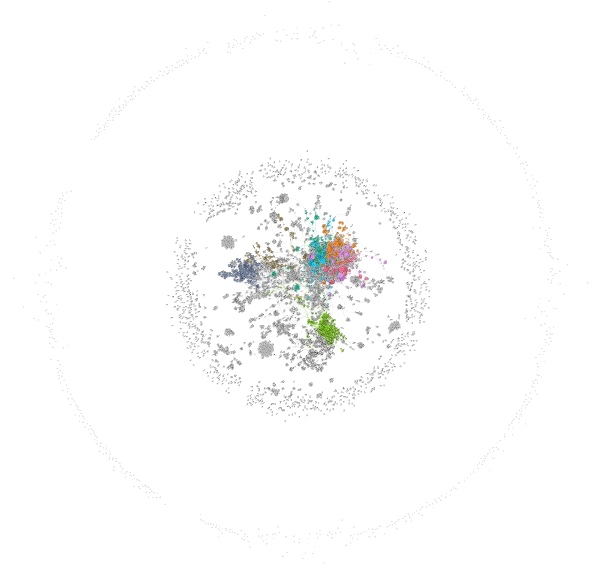
\includegraphics[width=\linewidth]{img/Final Graph.png}
  \caption{The Network of Artist Collaborations, Coloured Based On Modularity Score}
  \label{fig:network-graph}
\end{figure}

We notice that there is a large weakly-connected component in the middle of the figure, surrounded by many isolated and small communities. They represent the artists that have decided to not interact much with their peers and be very selective in choosing who to collaborate with, having only 2-3 connections. 

In the bigger component, we notice that some communities stand out; the artists that are part of these communities are the ones which collaborate the most with each other. The communities are not clearly separated, meaning that the artists tend to work with other artists which may not belong to the usual genre in which they can be found (an interesting example in this case is Ozzy Osbourne, who appears to have collaborated with Post Malone and Travis Scott during his career). 

There are also some tightly-knit communities (highlighted in Figure \ref{fig:focus}), which are separated or very weakly connected to the main component. They are made of artists that collaborated on the same songs almost exclusively, having no connection to the rest of the artists whatsoever (the rightmost community), or are connected by only one individual (leftmost community, through David Alvarez).

\begin{figure}[h]
  \centering
  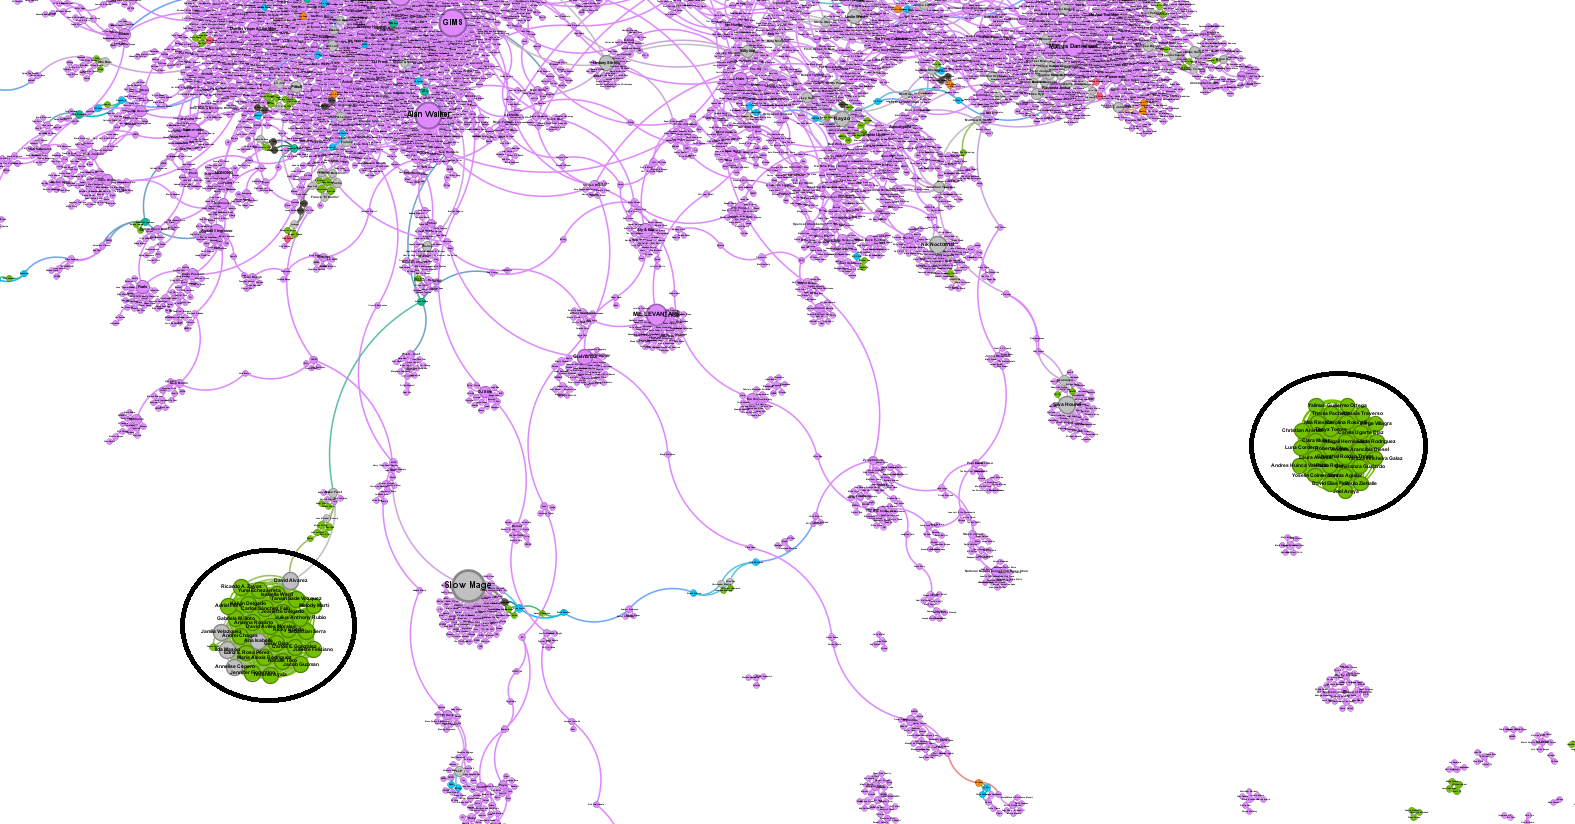
\includegraphics[width=\linewidth]{img/focus.png}
  \caption{Focusing On The Tightly-Knit Communities (circled) Of The Network: Coloured Based On Clustering Coefficient}
  \label{fig:focus}
\end{figure}

\subsection{Network Overview}
In Table \ref{tab:metrics} we can observe some statistics related to the network, nodes and connected components.

\begin{table}[h!]
  \caption{A Network Overview}
  \label{tab:metrics}
  \begin{tabular}{| l | r |}
    %\centering
    \hline
    Avg. Degree: &         2.12 \\
    \hline
    Network Diameter: &       26 \\
    \hline
    Graph Density: &       0.000 \\
    \hline
     Connected Components: &      1722 \\
    \hline
\end{tabular}
\end{table}

The average degree of the graph is 2.12, which means that the network is sparse and there is a low connectivity among the artists (on average, an artist is connected to 2 or 3 other artists). Figure \ref{fig:degree-distribution} presents the degree distribution of the nodes.

\begin{figure}[h]
  \centering
  \includegraphics[width=\linewidth]{img/degree-distribution.png}
  \caption{Degree Distribution}
  \label{fig:degree-distribution}
\end{figure}
We notice that many nodes have extremely low degrees: around 7000 nodes have degrees less than 3. However, a few nodes prove to have very high degrees: the hubs, i.e. the artists with the most connections in the network, have, on some occasions more than 40 collaborators for their songs, some of them even surpassing 70.

The sparsity of the graph is supported by its density, which, according to Gephi, has the value 0.000, meaning that the value is so low that this was the best approximation it could find. Knowing that the number of nodes is N = 11488 and the number of edges is E = 12148, we can check the accuracy of this result by applying the known formula of the average density of a graph ($density = \frac{2E}{N(N-1)}$), we get the exact value 0.00018411.

The diameter of the network has the value 26, which highlights the sparsity of the network, while providing insight into how far apart the artists are from one another. It turns out that the largest shortest distance between two artists is of 26 connections which, considering the high number of nodes and edges in the network, is quite small. However, this metric does not take into account the fragmented components of the network, which make up a considerable part of the total network. 

In Figure \ref{fig:closeness-centrality}, we can see the distribution of the closeness centrality values of the nodes. This plot shows that there are over 1600 nodes that have a closeness centrality value of 1, meaning that they are key nodes in the network which are close to most of the other nodes. These are the artists which have collaborated with so many people throughout their career that they have, on average, close ties to most of the other artists in the network. On the other hand, there are many nodes with low closeness centrality values, represented by the mass of points in the left side of the plot, closer to 0.

\begin{figure}[h!]
  \centering
  \includegraphics[width=\linewidth]{img/Closeness Centrality Distribution.png}
  \caption{Closeness Centrality Distribution}
  \label{fig:closeness-centrality}
\end{figure}

It appears that we have 1722 connected components in the network, which accounts for a highly disconnected graph, with 1722 isolated communities. This comes as no surprise if we look at the considerable number of small communities that encircle the bigger cluster in the center of Figure \ref{fig:network-graph}. This means that there are some artists which are more selective with the connections they make, and they keep these connections inside their inner circle.

\subsection{Community Detection}

We detected 1769 communities in this network, with modularity 0.937, with sizes plotted in Figure \ref{fig:modularity}.

\begin{figure}[h!]
  \centering
  \includegraphics[width=\linewidth]{img/communities-size-distribution.png}
  \caption{Size Distribution With Respect To Modularity}
  \label{fig:modularity}
\end{figure}

Such high modularity refers to the fact that this network is densely connected within the communities, but the communities are sparsely connected with each other. This means that artists tend to stick to collaborations inside their communities and do not venture much outside of them. The great variety in values in the plot from Figure \ref{fig:modularity} comes from the fact that the communities that are part of the circle that can be seen in Figure \ref{fig:network-graph} have a few connections between them, but the nodes that are part of these communities have connections from one to another in most cases.

\subsection{Node and Edge Overview}

Table \ref{tab:node-edge-metrics} presents some insights related to the nodes and the edges of the network, namely the average clustering coefficient and the average path length.

\begin{table}[h!]
  \caption{Node \& Edge Overview}
  \label{tab:node-edge-metrics}
  \begin{tabular}{| l | r |}
    \hline
    Avg. Clustering Coefficient: &         0.146 \\
    \hline
    Number of Triangles: &                 7704 \\
    \hline
    Avg. Path Length: &                    9.37 \\
    \hline
\end{tabular}
\end{table}

An average clustering coefficient of 0.146 means that, on average, a node forms connections with around 14\% of its neighbours, which means that there is a moderate level of local clustering in the network. We can deduce that artists have a tendency of sticking together with their neighbours, but not to an extremely high degree. There are 7704 triangles found in the network, which supports the local connectedness of the network. 

The average path length of 9.37 means that, in order to arrive from one artist to another in a network, one needs to visit, on average, around 10 other artists. This means that the network of artists presents some degree of connectivity, albeit not a high one.

\subsection{Comparison with ER}

We are going to build an Erdos-Renyi network having the same number of nodes (11488) and edges (12148) as our network. This means that the probability of two nodes being connected is 0.00018. A representation of the ER network with these properties can be seen in Figure \ref{fig:ER-graph} and in Table \ref{tab:ER-metrics} we store an overview of the this network.

\begin{figure}[h!]
  \centering
  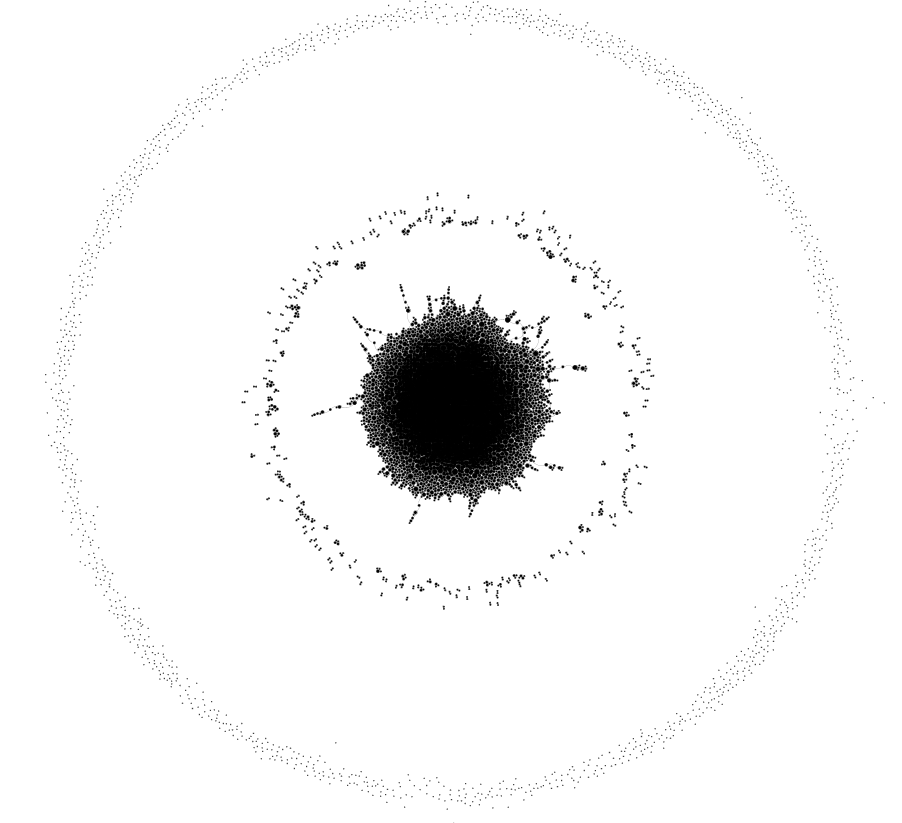
\includegraphics[width=\linewidth]{img/ER_graph.png}
  \caption{Erdos-Renyi Graph Having The Same Number Of Nodes As The Artists Network}
  \label{fig:ER-graph}
\end{figure}

\begin{table}[h!]
  \caption{ER Network Overview}
  \label{tab:ER-metrics}
  \begin{tabular}{| l | r |}
    %\centering
    \hline
    Avg. Degree: & 2.072 \\
    \hline
    Density: & 0.00018 \\
    \hline
    Avg. Clustering Coefficient: & 0.0 \\
    \hline
    Number of Triangles: & 1 \\
    \hline
    Connected Components: & 1747 \\
    \hline
    Avg. Path Length: & 12.012 \\
    \hline
    
\end{tabular}
\end{table}

We notice that the average degree in the ER graph is 2.072, which is less than the average degree of the artists network, which is 2.12. The 0.048 difference represents the fact that, on average, the the ER graph is still sparse and its level of connectivity is even less than the one of our network.

The density of the ER network is extremely low as well, as expected, which is means that the two networks have extremely similar densities, but the ER network proves to be ever-so-less-dense than the other, under very close analysis.

The average clustering coefficient of the ER network is 0.000, which means once again that the actual value is extremely low. The number of triangles in this case is 1, which is significantly lower than in the case of the artists network. This means that in the ER network there is no clustering and there are very few connections among the neighbours of the nodes.

There are 1747 connected components in the ER network, 25 more than in the case of our network. This implies that there is an even bigger number of isolated communities than in the case of the first network; if we look at the representation from Figure \ref{fig:ER-graph}, we notice that the outer ring around the central agglomeration of nodes is thicker compared to the one of the artists network.

\subsection{Comparison with BA}

In this section, we are going to compare the artists network with the Barabasi-Albert network composed of the same number of nodes(10721). The number of links m that connect a newly-added node to the nodes that are already in the network are computed using the formula $m=\frac{E}{N}$, which, in our case, means that $m=1$. In Table \ref{tab:BA-metrics} there are some metrics describing the BA network.

\begin{table}[h!]
  \caption{BA Network Overview}
  \label{tab:BA-metrics}
  \begin{tabular}{| l | r |}
    %\centering
    \hline
    Avg. Degree: & 1.9998 \\
    \hline
    Density: & 0.000174 \\
    \hline
    Avg. Clustering Coefficient: & 0.0 \\
    \hline
    Number of Triangles: & 1 \\
    \hline
    Connected Components: & 1 \\
    \hline
    
\end{tabular}
\end{table}

We notice that the average degree in the case of the BA model is less than the one of the artists network having the same parameters. This means that, on average, a node in the BA network is connected to less nodes than in the other graph. 

The low density supports the small connectivity in the BA model: not only is it extremely low, but it is also lower than the one of our graph. This means that the BA network is even sparser than the network of artists.

The number of triangles found in the network accounts for the fact that the average clustering coefficient is 0, meaning that the neighbours on a node don't have the tendency of forming connections. They tend to be more independent.

\begin{figure}[h!]
  \centering
  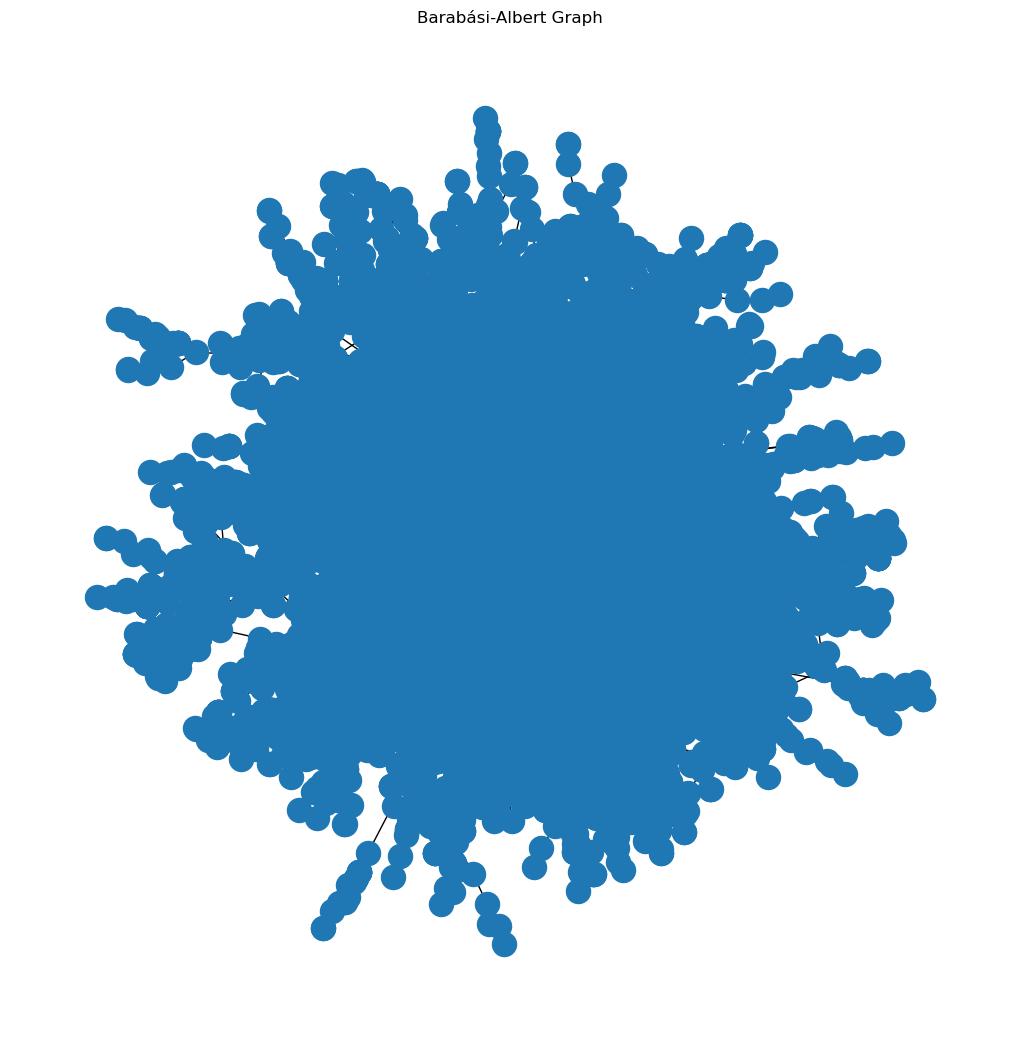
\includegraphics[width=\linewidth]{img/BA_graph.png}
  \caption{Barabasi-Albert Network Having The Same Number Of Nodes As The Artists Network}
  \label{fig:BA-network}
\end{figure}

In what concerns the number of connected components, so far the BA model has the lowest value, which is 1; we deduce that the BA network is one big weakly-connected component. As a rough visual representation made in Python, Figure \ref{fig:BA-network} depicts the BA network; we can clearly see that there are no more isolated components and, instead, all the nodes are part of the concentrated mass of points.

\section{Open Question}

So far, We have analysed a network of artists connected by songs they worked on together. In this section, we will use the results of the analysis to find an answer to the following question:

\textit{Are the artists with the most collaborations more popular than the ones who prefer to have less collaborations?}

For this task, we will use the \textit{popularity} column of the nodes dataset. Popularity is defined as an integer value between 0 and 100, where 0 is the least popular and 100 the most popular. The popularity of an artist is computed based on the popularity of all their tracks \cite{GetArtist}. We will look for the nodes with the highest degrees (high degree means many collaborations) and compare their popularity index with their size.

First, we will re-draw the network, focusing on the central component, where there are the most nodes and the most connections. In Figure \ref{fig:network-heatmap-artists-labels}, we have used a heatmap-style colour palette to represent the popularity of the artists: the darker the colour, the more popular the artist. For a better understanding, we changed the labels from the names of the artists into the artist's popularity and represented the result in Figure \ref{fig:network-heatmap-popularity-labels}.

\begin{figure}[h!]
    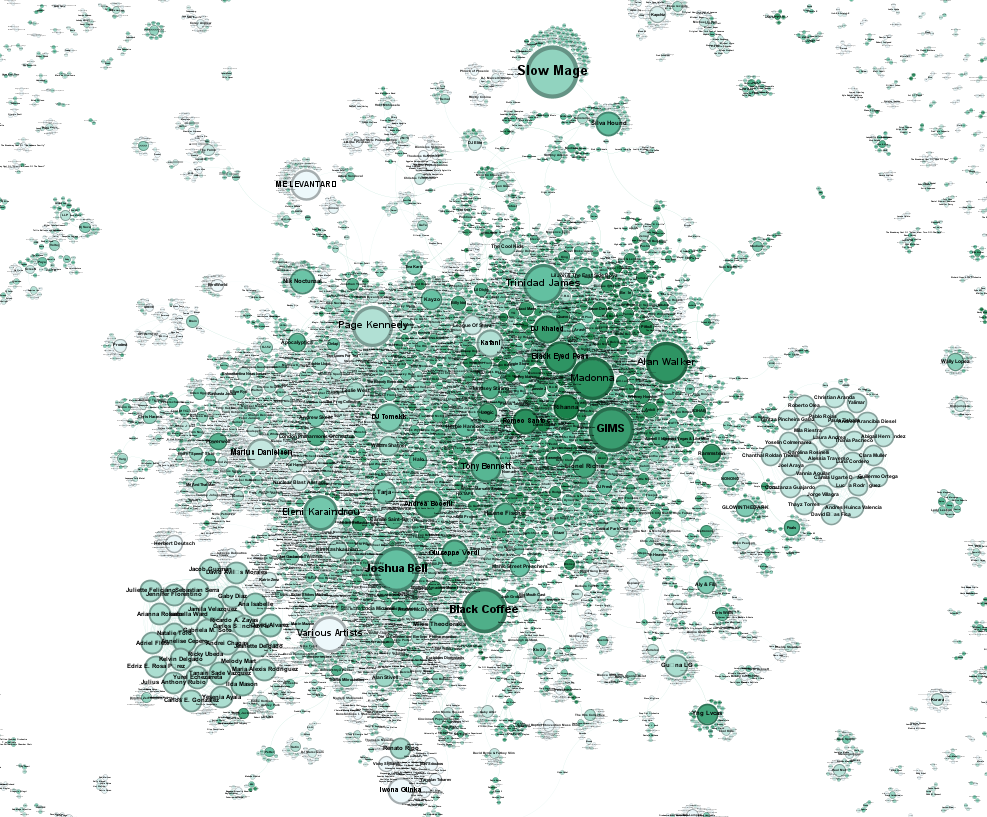
\includegraphics[width=\linewidth]{img/Network_Heatmap_for_Popularity_WIth_Labels.png}	
    \caption{The network of artists: the size of the nodes is proportional to their degree (i.e. how many collaborations they have) and the colour scheme is a heatmap for the popularity feature. The labels are the names of the artists}
    \label{fig:network-heatmap-artists-labels}
\end{figure}

\begin{figure}[h!]
    \centering
    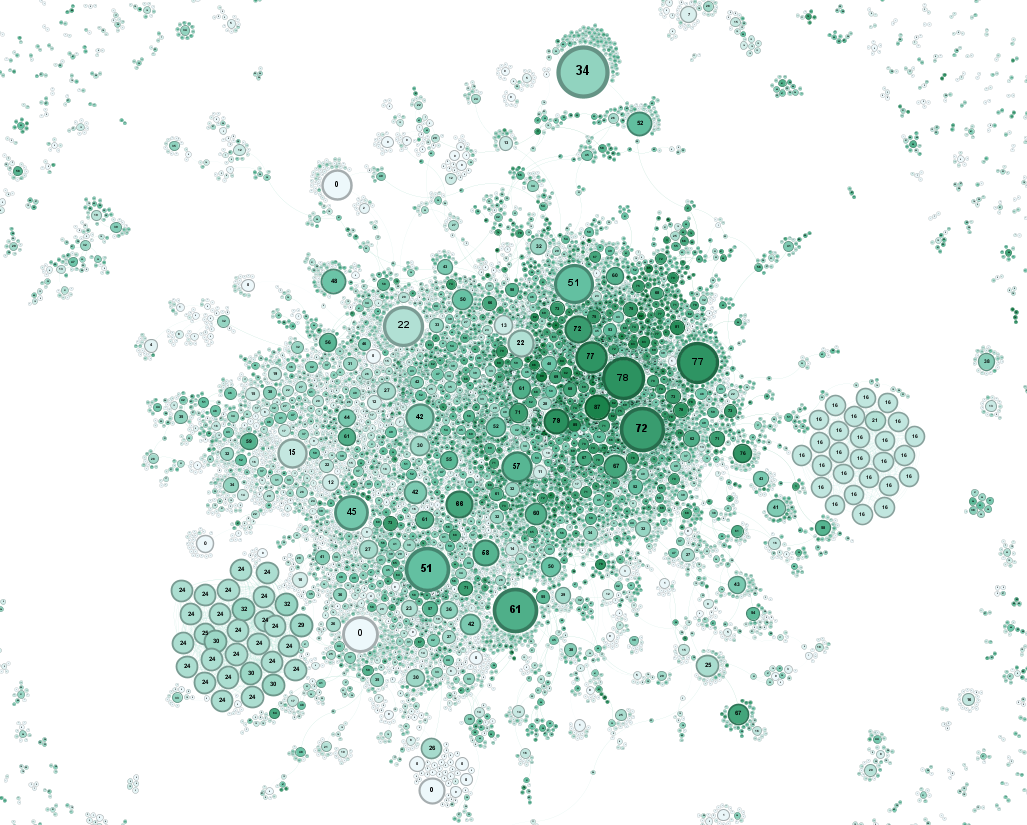
\includegraphics[width=1\linewidth]{img/Network_Heatmap_for_Popularity_WIth_Labels(popularity).png}
    \caption{The same network of artists as in Figure \ref{fig:network-heatmap-artists-labels}, this time having as labels the popularity index of each artist}
    \label{fig:network-heatmap-popularity-labels}
   
\end{figure}

We notice that the artists with the most collaborations that stand out the most are: Slow Mage, Page Kennedy, Trinidad James, DJ Khaled, Black-Eyed Peas, Madonna, Alan Walker, GIMS, Black Coffee and Joshua Bell. If we look at their popularity, we notice that Slow Mage, the artist with the most number of collaborations, has a popularity of only 34. Some research on this artist revealed that they actually make slow+reverb remixes of songs, which accounts for the low popularity: not many people actively look up remixes on Spotify. The reason why this artist has so many collaborations is due to the fact that they have different artists performing every song before adding any effects to them. The same goes for Black Coffee: he is an African DJ who has gained greater popularity due to the fact that he managed to gain the Guinness World Record for longest-ever DJ set.

In what concerns the other artists, we notice that they have a pretty high popularity index, as well as a good number of collaborations. GIMS, Alan Walker and Madonna, for example, have 72, 77 and 78 popularity, respectively, which are all values close to 100 and way above the average. In fact, most of the nodes with high degrees have a medium-to-high popularity index, with only some exceptions, like Slow Mage. What seems to be common for all these nodes is the fact that, apart from the large number of connections, they appear to be connected to nodes having a reasonably high popularity index. For example, GIMS has among his connections the famous singers J Balvin, Pitbull and Maluma, who have popularity 83, 81 and 81, respectively.

There is only one maximal popularity value in this dataset, and it belongs to Taylor Swift. However, she has only around 20 collaborators, some of which having not been included in this dataset, so this might be a reason why she is not so visible in the network.

It appears that, for most of the cases, the number of collaborations helps artists become more popular. There are some outliers who make it big mostly on their own (Taylor Swift), or who have many collaborations, but, despite this, not manage to gain too much popularity out of it (Slow Mage). However, for the larger majority, we can say that having many connections helps in soaring in popularity, so long as these connections have, themselves, a reasonable amount of popularity (i.e. the connections are meaningful from the point of view of the popularity).

%{What would happen if the artists with the most collaborations would be removed from the equation? How fast would the network become disconnected? We will remove the nodes with the degrees greater than or equal to 50 and we will check}%


\section{Discussion}
% actually the conclusion and future work (comment by me)
We have analysed a network of artists with varying degrees of popularity who were connected to each other based on songs they have worked on together. We have seen that, most of the time, having many collaborations influence the level of popularity that an artist has, but it is not a sufficient condition. Some artists manage to "make it big" without too much help from others, but there are also some who, despite having a very large number of connections, cannot make it to the top. All in all, having a considerable number of qualitative collaborators on your songs (i.e. other popular or very popular artists) provides a small push towards increasing your popularity level on Spotify.

As future work, we could analyse how the genres with which the artists interact influence their own style. In addition, we could check connected the network is after removing the most popular artists, compared to removing those with the most collaborations.

% The next two lines define the bibliography style to be used, and the bibliography file.
\bibliographystyle{ACM-Reference-Format}
\bibliography{biblio}

\end{document}

